\chapter{Random Circuit Sampling}

Despite four decades
of research in the field of quantum computing, 
there was no physical proof whether it would be possible to realise quantum computers
which have an advantage over classical ones. This only changed
recently, when a team from Google and the UCSB claimed to have demonstrated \textit{quantum supremacy}
with a 54 superconducting qubit quantum processor \cite{martines2019supremacy}. For this purpose, they
chose the problem of \textit{random circuit sampling}, a problem specificaly designed
as a quantum supremacy experiment \cite{Boixo2018supremacy}.

This chapter will motivate and introduce the theoretical framework of random circuit
sampling, also used as the benchmark for Restricted Boltzmann machines in this
study. Further, the results of Google's quantum supremacy experiments and their
implications for the (near) future of quantum computing will be discussed.

\section{Quantum Supremacy}

The term \textit{quantum supremacy} has been coined by John Preskill in 2012
\cite{preskill2012quantum}. It describes the point in time when a physical quantum computer
outperforms a classical computer on some task for the first time. The problem
solved by the quantum computer does not need to be useful. Its only purpose is
to proof that a quantum computer can be realised that has an advantage over
classical computers on \textit{some} problem.

There exist different proposals for quantum supremacy
experiments. Since quantum computers don't promise to outperform classical
computers on every problem, as discussed in section \ref{}, but only provide a
practical advantage for problems which lie in \textbf{BQP} and outside of
\textbf{P}, quantum supremacy experiments must be based upon a strong theoretical foundation.

One way to demonstrate quantum supremacy would be to run Shor's
algorithm for integer factorisation \cite{shor1997factorisation} on a physical quantum computer on some number which would not be feasible
to decompose with known classical algorithms on existing supercomputers. The issue with this approach is that many
qubits are necessary to represent such numbers while today it's possible to
build quantum processors with about 50 qubits of reasonalble quality.

Another famous proposal for a quantum supremacy experiment is \textit{Boson Sampling}, which is based on the
fact that calculating the permutant of a matrix is computationaly hard \cite{aaronson2013boson}.

The approach that a team from Google and UCSB took last year is called \textit{Random
  Circuit Sampling} (RCS). In this approach, random quantum circuits of specific structures which create highly
entangled states are run on a quantum processor and are simulated classically. For
enough qubits and depth, performing the classical simulations would take years 
even on the biggest existing supercomputers. If the quantum computer can generate outputs
for such circuits which cannot be simulated classically anymore while their output can still be
verified to be correct, this would demonstrate quantum supremacy. A metric that
allows the verification on random circuit instances which cannot be simulated is
the \textit{cross entropy fidelity}.

\section{Cross Entropy Fidelity}

The challenge of quantum supremacy is that one has to be able to verify the
results of the quantum computer on instances which cannot be calculated
classically anymore. In the case of integer factorisation, this is a simple task
as the test for the correctness consists of simple multiplications which can be
performed efficiently. Since integer factorisation needs more qubits than
currently available in existing quantum computer hardware, other supremacy
experiments like RCS provide a framework to demonstrate quantum supremacy much
earlier.

The first observation to undertand the concept of RCS is that every quantum
circuit acting on $n$ qubits can be described by a single $2^n$ dimensional
unitary matrix, as illustrated in figure~\ref{circuitasunitary}. This follows
from the fact that quantum gates are described by unitary transformations and
the matrix product as well as the tensor product of two unitaries is a unitary again.

\begin{figure}[H]
  \begin{equation}
      \Qcircuit @C=1em @R=1em {
        & \ctrl{2} & \qw & \gate{H} & \ctrl{1} &
        \gate{H} & \qw \\
        & \qw & \ctrl{1} & \gate{H} & \targ &
        \gate{H} & \qw \\
        & \targ & \targ & \gate{Z} & \qw & \ctrl{-1} &
        \qw
      }
      =
      \Qcircuit @C=1em @R=0em {
        & \multigate{2}{U} & \qw \\
        & \ghost{U} & \qw \\
        & \ghost{U} & \qw
      } 
    \end{equation}
    \label{fig:circuitasunitary}
  \caption{Every Circuit can be described by one big unitary acting on $n$
    qubits. W.l.o.g. the resulting states corresponds to the first row of the
    unitary $U$.}
\end{figure}

A quantum circuit consisting of gates chosen uniformly at random thus
will act like a uniformly random unitary $U$. Since the input state of the circuit can be assumed to be
initialised in the $\Ket{0^{\otimes n}}$ state, the amplitudes of the final
quantum state of the circuit correspond to the first row of the random unitary $U$.

The entries of this row are complex numbers with real and imaginary parts
distributed by an unbiased Gaussian with respect to the normalisation constraints.
The output probablities of the random circuit are given by
the squared norms of these entries.
They are thus distributed as the square of
a Gaussian distribution which is an exponential distribution,
also known as a Porter-Thomas distribution \cite{Porter1956Fluctuations}. So the probablities $p(x_j) =
\| \Braket{x_j\psi_{RC}} \| ^2$ to observe bitstrings $x_j \in \{x_j\}_{j=1}^N$ with
$N=2^n$ are distributed according to

\begin{equation}
  Pr(p) = e^{-Np}
\end{equation}

as visualised in figure~\ref{fig:porterthomas}.

\begin{figure}[H]
  \label{fig:porterthomas}
  \centering
  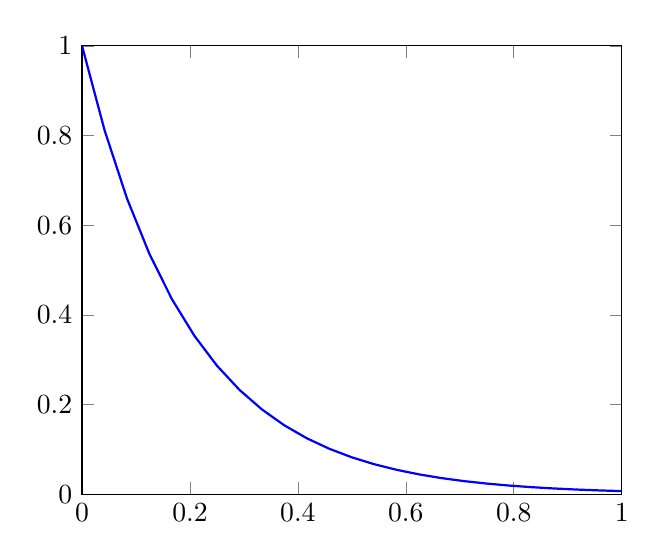
\begin{tikzpicture}
    \begin{axis}[
      xmin=0,
      ymin=0,
      xmax=1,
      ymax=1]
      \addplot[blue, domain=0:1, thick] {e^(-5*x)};
    \end{axis}
  \end{tikzpicture}
  \caption{Distribution $P(p_{x_j})$ of output probablities $p_{x_j}$ of a
    quantum circuit. The distribution $P(p_{x_j})=e^{-Np}$ is distributed as
    Porter Thomas. A lot of output strings will have a low probablity to be
    observed and a few output strings will dominate the observed outputs.}
\end{figure}

As quantum computers suffer from decoherent noise, it is
important to undestand how noise during the computation influences the output
distribution from the quantum computer and if noisy quantum computers can still
outperform classical computers on the RCS task. Knowing that the outputs are
Porter Thomas distributed will help with that.

The task is to understand how samples $S=\{x_1,\dots,x_m\}$ drawn from a perfect execution of
$U$ compare to a set $S^{\prime}=\{x_1^{\prime},\dots,x_m^{\prime}\}$ of samples drawn from a potentially noisy
execution of $U$.

A well motivated measure for the difference between the underlying
probablity distributions $p_U$ and $p_U^{\prime}$ of samples $S$ and $S^{\prime}$ is the \textit{cross entropy}, defined as


\begin{equation}
  H(p_U^{\prime},p_U) = - \sum_{j=1}^Np_U^{\prime}(x_j|U) \log{p_U(x_j)}.
\end{equation}

Of interest is the expected quality of the potentially noisy execution over
different random circuit instances:

\begin{equation}
  \mathbb{E}_U[H(p_U^{\prime},p_U)] = \mathbb{E} [\sum_{j=1}^Np_U^{\prime}(x_j|U)\log{\frac{1}{p_U(x_j)}}].
\end{equation}

In a worst case, the output of the noisy execution can be assumed to
be statistically uncorelated with the output of the perfect execution. Thus,
and since the output distribution for a fixed $x_j$ over many random circuit
instances $U$ also has the shape of the Porter-Thomas distribution \cite{harrow2008random},
$-\mathbb{E}_U[\log{p_U(x_j)}]$ can be computed independently as: 

\begin{align}
  -\mathbb{E}_U[\log{p_U(x_j)}] &\approx - \int_0^{\infty}Ne^{-NP}\log{p} dp \\
                                &= \log{N} + \gamma,
\end{align}

where $\gamma \approx 0.577$ is the Euler constant.
Using the fact that $\sum_{j=1}^Np_U^{\prime}(x_j) = 1$ for any distribution $p_U{\prime}$, the average cross
entropy $\mathbb{E_U}[H(p_U^{\prime},p_U)]$ between the Porter-Thomas distribution and any other uncorrelated distribution is
given as 

\begin{equation}
  \mathbb{E}_U [H(p_U^{\prime},p_U)] = \log{N} + \gamma.
\end{equation}

This is equivalent to the cross entropy $H_0 = \log{N} + \gamma$ between the
Porter-Thomas and the uniform distribution. This means that in the worst case on
average a noisy execution will be as good compared to a perfect execution as sampling
every bitstring with probablity $1/N$. $H_0$ differs from the entropy $H(p_U)$ of
the Porter-Thomas distribution, which corresponds to the cross-entropy with
itself

\begin{align}
  H(p_U) &= - \int p N^2e^{-Np}\log{p} dp \\
         &= \log{N} -1 + \gamma,
\end{align}

only by a $-1$ term. 

This directly leads to a benchmark for any algorithm $A_U$ sampling output strings from a
random circuit $U$, given either by a
classical simulation or by a (noisy) quantum computer. The quality of 
$A_U$ can be calcuated as the difference between
the entropy of the uniform distribution and the cross entropy of the output
samples from $A_U$ with the Porter-Thomas distribution. This metric is
defined as the \textit{cross entropy difference} \cite{Boixo2018supremacy}:

\begin{align}
  \Delta H(p_A) &\equiv H_0 - H(p_A, p_U) \\
                 &=\sum_j (\frac{1}{N} - p_A(x_j|U))\log{\frac{1}{p_U(x_j)}}.
\end{align}

This metric is zero for an algorithm sampling from the uniform
distribution and one for an algorithm sampling from the underlying Porter-Thomas
distribution of the circuit.
Notice that in order to calculate $\Delta H(p_A)$, 
a perfect simulation of the random circuit is necessary 
as the values of $p_U(x_j)$ have to be known. This is not possible in the quantum
supremacy regime. As discussed shortly, it will be possible
to extrapolate the cross entropy difference of $A_U$ to the quantum supremacy regime with high
precision based on samples of its cross entropy difference on smaller circuit
instances which can still be simulated classically.

Another justification for the cross entropy difference is that the $l_1$ distance between the uniform and Porter Thomas distribution

\begin{align}
  l_1(p,q) &= \| p-q\|_1 \\
           &= \sum_{j=1}^N \mid p_i - q_i \mid
\end{align}

is a constant and thus independent of the number of qubits $n$. Therefore a
constant number of samples is sufficient to calculate the cross entropy
difference.

The experimental cross entropy difference of $A$

\begin{equation}
  \alpha = \mathbb{E}_U[\Delta H(p^{\prime}_U)]
\end{equation}

can be obtained by the execution of several random circuits $U$. Quantum
supremacy is achieved by a physical quantum computer when its average cross
entropy

\begin{equation}
  1 \geq \alpha > C
\end{equation}

is greater than the average perfomance $C$ of the best known classical algorithm $A^*$:

\begin{equation}
  C = \mathbb{E}_U[\Delta H(p^*)] .
\end{equation}

In the regime where perfect simulations are possible, $C=1$ and quantum
supremacy cannot be achived. For sufficiently many qubits, perfect simulations
will not be possible anymore and $1 > C \geq 0$ with $C$ decreasing exponentially
with the number of gates $g>>n$. For a typical set of samples $S_{exp}$ drawn from the
execution of a quantum circuit, the central limit theorem implies that

\begin{equation}
  \label{eq:cef}
  \alpha \simeq H_0 - \frac{1}{m} \sum_{j = 1}^m \log{\frac{1}{p_U(x_j^{exp})}}.
\end{equation}

The statistical error in this equation grows like
$\frac{\kappa}{\sqrt{m}}$ with $\kappa=1$.

The experimental setup to estimate the cross entropy difference of any
approximate simulation of a quantum computer thus is:

\begin{enumerate}
\item Select random circuit $U$.
  \item Take sufficiently many samples $S_{exp} = \{x_1, \dots, x_m\}$, m in
    range $10^3-10^6$.
    \item Compute the quantities $\log{\frac{1}{p_U(x_j^{exp})}}$ with the aid
      of a sufficiently large quantum computer.
      \item estimate $\alpha$ using equation~\ref{cef}.
\end{enumerate}

\section{Extrapolating to the Supremacy Regime}

Keeping the qubits in a coherent state during a calculation and applying quantum
gates exactly is a difficult task. Qubits will suffer from decoherent noise
which will destroy the quantum states. This will happen in particular in early
implementations of quantum computers. The quality of the
qubits and gate applications is expected to improve over time.

Before large scale error-corrected quantum computers will be available, so
called noisy intermediate scale qantum (NISQ) computers present the first stage
of quantum computing hardware. Such noisy devices will already provide an
advantage over classical computers on specific problems. If the noise can be
kept below a certain treshold, a NISQ device can be used to demonstrate quantum
supremacy on the RCS task.

In the presence of noise, the quantum state $\rho$ generated by a physical quantum computer
after the execution of a random circuit $U$ can be represented as

\begin{equation}
  \rho = \tilde{\alpha} U \Ket{\psi_0} \Bra{\psi_0} U^{\dagger} + (1- \tilde{\alpha}) \sigma
\end{equation}

with $\tilde{\alpha}$ being the circuit \textit{fidelity} and $\sigma$ being an orthogonal state to the true state
$\Bra{\psi_0}U^{\dagger}\sigma U \Ket{\psi_0} = 0$.
The corresponding average cross entropy difference then is:

\begin{align}
  \alpha &= \mathbb{E}_U[H_0+ \sum_j \Bra{x_j} \rho \Ket{x_j} \log{p_U(x_j)} ] \\
         &= \tilde{\alpha} + (1-\tilde{\alpha})H_0 + \mathbb{E}_U[(1-\tilde{\alpha}) \sum_j \Bra{x_j} \sigma \Ket{x_j} \log{p_U(x_j)}].
\end{align}

The states generated by the random circuits are
maximally entangled. A single bit or phase flip introduced by an additional $X$
or $Z$ gate in the circuit completely destroys such a state. Instead of being
Porter Thomas distributed, the output with an additional $X$ or $Z$ gate at any
position would be almost uniformly distributed as shown in figure~\ref{fig:rcs_noise}.

\begin{figure}[H]
  \centering
  \label{fig:rcs_noise}
  \includegraphics[width=0.58\textwidth]{figures/rcs_noise}
\end{figure}

In other words, it is not possible to infer any information about the output
probablites without a perfect simulation of the circuit.
This justifies the assumption that the true output probablities and the output
of the quantum computer are (almost) uncorrelated.
This assumption of uncorrleation in turn leads to the conclusion that the
circuit fidelity $\tilde{\alpha}$ of a random
circuit $U$ is approximately equal to the average cross entropy

\begin{equation}
  \label{eq:extrapolate}
  \alpha = \mathbb{E}_U[\Delta H(p_{exp})] \approx \tilde{\alpha}.
\end{equation}

This means that the fidelity $\alpha$ of a quantum device can be extrapolated to
the quantum supremacy regime withe estimates of it on random circuit instances
which can still be simulated classically.

Even further, this also means that the cross entropy difference can also aid to estimate
the single and two qubit gate and errors of a quantum device:

\begin{equation}
  \alpha \approx e^{-r_1g_1 - r_2g_2 -r_{init}n -r_{mes}n}
\end{equation}

with $r_1, r_2 \ll 1$ being the Pauli error rates for 1 and 2 qubit gates, $r_{init},
r_{mes} \ll 1$ the initialisation and measurement error and $g_1,g_2 \gg 1$ being the
numbers of 1 and 2 qubit gates. This relation has been numerically confirmed by
Boixo et al. \cite{Boixo2018supremacy}, indicating that the relation between the
cross entropy difference and the circuit fidelity can be used to extrapolate the
cross entropy difference of a quantum device to the quantum supremacy regime.

So, even with a noisy quantum computers it is possible to demonstrate quantum
supremacy, i.e. to approximate the output distribution of random circuit instances
better than possible by any classical algorithm known, by
calculating the fidelity on random circuit instances still possible to simulate
classically and extrapolating it to the supremacy regime using
equation~\ref{eq:extrapolate}.
If the fidelity is greater zero in the regime where no classical simulation is possible anymore,
quantum supremacy has been demonstrated.

\section{Random Circuit Design}

The derivation of the cross entropy difference based on the assumption that the
output probablities of random circuit instances will be distributed according to
the Porter-Thomas distribution. As it is known that circuits of low depth as
well as so called \textit{Clifford Circuits} can be simulated classically
efficiently, it is crucial to understand which requirements the structures of
the random circuits has to fulfil in order to be hard to simulate classically and generate
exponential output distributions.

In a fully connected architecture, random circuits approximate a pseudo-random
distribution with logarithmic depth. Fully connected in this statement means
that 2 qubit gates can be applied to pairs of any two qubits of the circuit. In
architectures like superconducting qubits as for instance Google's Sycamore
processor the qubits are lied out on a 2D lattice, allowing 2 qubit gates only
to be applied to neighbouring qubits on that lattice. Circuits on fully
connected architectures of logarithmic dephts are known to be translatable into
circuits of depht $\sqrt{n}$ on 2D lattices. Boxio et al. used numerical
simulations to optimized strategies to generate random circuits with minimized
time to converge to a Porter Thomas distribution leading to the following algorithm:

\begin{enumerate}
  \item Initialize in the state $\Ket{0}^{\otimes n}$.
  \item Apply a Hadamard gate to each qubit.
  \item Apply a random circuit with a stack of depth $d$, where each layer has
    the following two clock cycles:
    \begin{enumerate}
      \item Apply a clock cycle of random single-qubit gates to all qubits.
        \item Apply a clock cycle of two-qubits gates.
    \end{enumerate}
\end{enumerate}

The gate set consists of the single qubit gates $\{\sqrt{X}, \sqrt{Y}, T\}$ with

\begin{equation}
  \sqrt{X} = \frac{1}{\sqrt{2}} \begin{pmatrix}
    1 & - i \\
    - i & 1
    \end{pmatrix}
\end{equation}

and

\begin{equation}
  \sqrt{Y} = \frac{1}{\sqrt{2}} \begin{pmatrix}
    1 & -1  \\
    1 & 1 
  \end{pmatrix}
\end{equation}

being the ``square root of $X$'' and the ``square root of $Y$'' gates:

\begin{align}
  \sqrt{X}^2 &= (\frac{1}{\sqrt{2}} \begin{pmatrix}
    1 & - i \\
    - i & 1
  \end{pmatrix})^2 \\
  &= \begin{pmatrix}
    0 & 1 \\
    1 & 0
  \end{pmatrix} \\
  &= X
\end{align}

and

\begin{align}
  \sqrt{Y}^2 &= (\frac{1}{\sqrt{2}} \begin{pmatrix}
    1 & -1 \\
    1 & 1
  \end{pmatrix})^2 \\
  &= \begin{pmatrix}
    0 & -i \\
    i & 0
  \end{pmatrix} \\
  &= Y.
\end{align}

The circuit can be seperated into different layers, where each layer consists of one
layer of $CZ$ gates and one layer of random single qubit gates. The single qubit
gates are chosen such that each single-qubit gate on qubit $q$ in the current
cycle differs from the single-qubit gate on $q$ at the previous cycle.

The 2-qubit $CZ$ gates are applied as demonstrated in figure~\ref{fig:czgates}.
Notice that it is not possible to apply a 2 qubit-gate to any two qubits in
current quantum devvices but only to neighbouring qubits.

\begin{figure}[H]
  \centering
  \label{fig:czgates}
  \includegraphics[width=0.58\textwidth]{figures/cz_order}
\end{figure}

Boxio et al. could numerically show that random circuits generated this way
generate output distribuions according to Porter Thomas after a square root
number of cycles in the number of qubits.

\section{Exeperiments on Real Hardware}

With an algorithm for the generation of random circuits and a metric for the
quality of an execution of such circuits at hand, a team from Google and the UCSB conducted a quantum
supremacy experiment on the 54 superconducting qubit \textit{Sycamore}
processor, shown in figure~\ref{sycamore}.

\begin{figure}[H]
  \centering
  \label{fig:sycamore}
  \includegraphics[width=0.58\textwidth]{figures/sycamore}
\end{figure}

For the experiments, circuits with $n=10$ to $n=53$ qubits and
$m=12$ to $m=20$ cycles have been used. The full cycles generated according to the procedure
given above can be classically simulated up to $n=53$ qubits with $m=14$ cycles
in a reasonable amount of time. Beyond that regime, simplified circuit
architectures, called \textit{elided} and \textit{patched}, in which the
circuit is split into two sub circuits with only low entanglement in the elidid and not
entanglement in the patched version, allowed the classical simulation for up to $n=53$ qubits with $m=20$ cycles to
verify the fidelity of the Sycamore processor. For every circuit paramters, 20
circuits have been generated. For each circuit, $0.5-2.5$ million samples have been drawn
from the quantum processor.

\begin{figure}[H]
  \centering
  \label{fig:supremacy_results}
  \includegraphics[width=\textwidth]{figures/supremacy_results}
\end{figure}

The team reports an average fidelity of $F_{XEB} > 0.1\%$ with $5\sigma$ confidence
for the largest elided circuits. All results fit the extrapolated expected
fidelity from smaller circuits, making the team conclude that similar fidelities
would be achived for the full circuits. As classical simulations of these
circuits would take up to 100,000 years according to the team with a hybrid
Schroedinger-Feynman algorithm, this would imply
that quantum supremacy has been achived. The reported fidelities of the quantum supremacy for
the different circuit sizes and depths are reported in figure~\ref{supremacy_results}.

Shortly after these results have been announced, researchers from IBM claimed that the classical simulations
for the full circuits on 53 qubits and 20 cycles could have been performed
on the Summit supercomputer within a few days only with an optimized memory
usage. Experimental proof for these claims is still to be given.

Even if these circuits can be simulated within a few days, the quantum
processor would still outperform the classical simulation as it only
takes about 200ms to generate the 2 million samples for those circuits from it. As quantum
supremacy is a loosely defined term, the discussion might continue wheter
quantum supremacy has been demonstrated by the Google and UCSB team. Nevertheless, it is
an impressive engineering achivement to build a quantum processor of 53 qubits
which can execute quantum circuits consisting of up to 1,113 single-qubit and
430 two-qubit gates. For the future, the Google teams expects a double exponential grow of the computational
power of quantum computers as the classical simulation costs grow exponentially
with the computational volume (gates and qubits) and quantum hardware
improvements will probably follow a quantum processor equivalent of Moore's law.

This study does not focus on quantum circuits running on physical quantum devices,
but rather on the classical simulation of it. New and improved classical
approximate simulations of quantum systems with neural networks recently proofed
to work well on many problem instances. 
Understanding their performance and needed computaional resources on
the RCS task might provide useful insights about the capabilities and
limitations of neural networks for the classical simulation of quantum systems.


